\documentclass[aspectratio=43]{beamer}

\usepackage{dtucolors}
\usepackage[T1]{fontenc}
\usepackage[utf8]{inputenc}
\usepackage[english]{babel}
\usepackage{pgfplots}
\pgfplotsset{compat=newest}
\usepackage{booktabs}
\usepackage{siunitx}
\usepackage{listings}
\usepackage{subfig} % for subfigures
\usepackage{caption}

% Listings
\lstset{
    basicstyle=\scriptsize\ttfamily,% the size of the fonts that are used for the code
    breakatwhitespace=false,          % sets if automatic breaks should only happen at whitespace
    breaklines=true,                  % sets automatic line breaking
    captionpos=b,                     % sets the caption-position to bottom
    commentstyle=\color{s14a},        % comment style
    deletekeywords={},                % if you want to delete keywords from the given language
    escapeinside={\%*}{*)},           % if you want to add LaTeX within your code
    frame=single,                     % adds a frame around the code
    keywordstyle=\bfseries\ttfamily\color{s09}, % keyword style
    language=Python,                  % the language of the code
    morekeywords={*,...},             % if you want to add more keywords to the set
    numbers=left,                     % where to put the line-numbers; possible values are (none, left, right)
    numbersep=5pt,                    % how far the line-numbers are from the code
    numberstyle=\sffamily\tiny\color{dtugray}, % the style that is used for the line-numbers
    rulecolor=\color{dtugray},        % if not set, the frame-color may be changed on line-breaks within not-black text (e.g. comments (green here))
    showspaces=false,                 % show spaces everywhere adding particular underscores; it overrides 'showstringspaces'
    showstringspaces=false,           % underline spaces within strings only
    showtabs=false,                   % show tabs within strings adding particular underscores
    stepnumber=1,                     % the step between two line-numbers. If it's 1, each line will be numbered
    stringstyle=\color{s07},          % string literal style
    tabsize=2,                        % sets default tabsize to 2 spaces
    title=\lstname,                   % show the filename of files included with \lstinputlisting; also try caption instead of title
}

\lstdefinestyle{usecase}{
  emptylines=1,
  breaklines=true,
  basicstyle=\ttfamily\color{black},
  escapeinside={@}{@},
  keywordstyle=\bfseries,
  morekeywords = {Scenario, Postconditions, Preconditions}
}

\lstdefinestyle{Dart}{
  language=Java, 
  emptylines=1,
  breaklines=true,
  escapeinside={@}{@},
  morekeywords = {async}
}

\definecolor{mygreen}{rgb}{0,0.6,0}
\definecolor{mygray}{rgb}{0.4,0.4,0.4}
\definecolor{mymauve}{rgb}{0.58,0,0.82}

% Define colors used for listings
\definecolor{dkgreen}{rgb}{0,0.6,0}
\definecolor{dkred}{rgb}{0.6,0,0}
\definecolor{gray}{rgb}{0.5,0.5,0.5}
\definecolor{mauve}{rgb}{0.58,0,0.82}

%Reuse images from thesis.
\newcommand{\imgdir}{../Thesis/img/}

\newcommand{\figdir}{./fig/}

% Latin Modern
\usepackage{lmodern}
% Verdana font type
%\usepackage{verdana}
% Helvetica
%\usepackage{helvet}
% Times (text and math)
%\usepackage{newtx, newtxmath}

\usetheme[department=compute]{DTU}

\title[Requirements as tests]{Requirements as tests}
\author{Kim Rostgaard Christensen}
\institute{Technical University of Denmark (DTU)}
\date{\today}
	
\newcommand{\tabitem}{{\color{dtured}$\bullet$} }

\begin{document}
\frame{
	\maketitle
}

\frame{
	\frametitle{Outline}
	\tableofcontents
}

\section{Problem domain}
%TODO Remember requirement documentation rot.
\subsection{Problem statement}
\frame{
	\frametitle{Problem statement}
	
	\begin{block}{High failure rate in software projects}
	  Causes points to requirements being:
		\begin{itemize}
			\item Incomplete
            \item Under-specified
			\item Unaligned
		\end{itemize}
		\begin{quote}
``Delivery decision was made without adequate requirements information \dots in 73\% of the [studied] failed projects\cite{verner2008}.''
		
		\end{quote}
	\end{block}
	
	\begin{block}{Concept: link requirements to implementation}
% Having the requirements decoupled from implementation leads to split-brain operations and error-prone manual review processes to assert that the two are in sync.
%Humans make a substantial amount of errors when performing repetitive tasks.
	\end{block}
	
}

\frame {
  \frametitle{Design goals}
  
  \begin{block}{}
Use cases are unstructured, lets keep them that way, and only add the minimal structure to enable test generation.
Use cases work, because they are a good, common, communication platform. They are simple, with a clear objective.
Supplementing them with too many new (unrelated to the original objective) concepts, or a structure that is too constraining will make them lose their primary focus, and value as communication platform.
  \end{block}
  
  \begin{block}{}
  Basics of verified communication; repeat what I said
 This is basically an echo. So the best way of verifying agreement is to have your work read back to you, This can be done very nicely by changing the representation. For instance, from a textual to a visual representation.
  \end{block}
}

\subsection{Problem scope}
\frame {
  \frametitle{Problem scope - anticipated}
% At first; I regarded this as a "small" project. But then... Communicate that this project was larger than anticipated.
  
\begin{figure}[!htbp]
\includegraphics[scale=0.6]{\figdir mountain-trivial}
\caption{Anticipated project size}
\end{figure}
}

\frame {
  \frametitle{Problem scope - actual}
% At first; I regarded this as a "small" project. But then... Communicate that this project was larger than anticipated.

\begin{figure}[!htbp]
\includegraphics[scale=0.6]{\figdir mountain-challenging}
\caption{Actual project size}
\end{figure}
}

%Add a section on literate programming.
% Wouldn't it be nice to be able to tell the computer what the expected behaviour would be? https://en.wikipedia.org/wiki/Literate_programming

%Remember a section on what is gained, and what is lost.

%On Use case design:
%I didn't want to fuck up use cases. They work in their current form, and people have tried to "fix" them, add formalism and such. But none of the effort have caught on.
%So in essence; keep the use case as they are, and "fix" as little as possible.

%TODO clairifications. Using different terminologies for the same thing. Check Test support tools/test support framework.

%-----------------------
% Proposed solution

\section{Proposed solution}
\frame {
  \begin{tikzpicture}[remember picture,overlay]
    \node[text=black, text opacity=1.0,
          font=\scriptsize] at (current page.center) {\Huge Proposed solution};
  \end{tikzpicture}
}


\frame{
  \frametitle{Flow}
  \begin{figure}[!htbp]
    \centering
    \includegraphics[width=0.7\textwidth]{\imgdir ideal_flow-padded}
    \caption{Ideal development flow}
  \end{figure}
}

\frame{
  \frametitle{Flow -- with feedback}
  
  \begin{figure}[!htbp]
    \centering
    \includegraphics[width=0.7\textwidth]{\imgdir ideal_flow-feedback}
    \caption{Ideal development flow}
  \end{figure}
}

\frame{
  \frametitle{Requirement/implementation Relationship}

  \begin{figure}[!htbp]
    \centering
    \includegraphics[width=0.5\textwidth]{\imgdir tests-relation-to-implementation}
    \caption{Concept of mapping from requirements to implementation}
    \label{fig:tests-relation-to-implementation}
  \end{figure}
}

\frame {
  \frametitle{Solution overview}
  \begin{itemize}
    \item Additional structure for use cases.
    \item Technique for mapping to implementation.
    \item Tool for writing and structuring use cases -- and generate tests from them.
  \end{itemize}
}

\frame{
  \frametitle{Project plot}

  \begin{figure}[!htbp]
    \centering
    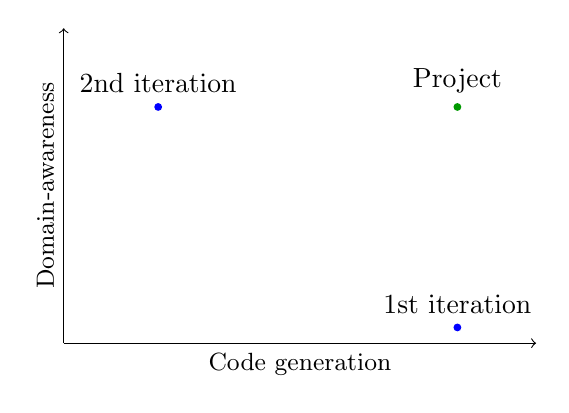
\begin{tikzpicture}
      % horizontal axis
      \draw[->] (0,0) -- (6,0) node[anchor=north,midway] {\small Code generation};

      % vertical axis
      \draw[->] (0,0) -- (0,4) node[anchor=south,rotate=90,midway] {\small Domain-awareness};

      \draw (5,0.2) node[circle,fill,inner sep=1pt, fill=blue, label=above:1st iteration] {};
      \draw (1.2,3.0) node[circle,fill,inner sep=1pt, fill=blue, label=above:2nd iteration] {};

      % Project dot
      \draw (5,3) node[circle,fill,inner sep=1pt, fill=dkgreen, label=above:Project] {}; 
    \end{tikzpicture}
    \caption{Project parameters and key points}
  \end{figure}
}

\frame {
  \frametitle{Origin}
  \begin{itemize}
    \item A mean for doing system-level testing
  \end{itemize}
}

\frame {
  \frametitle{Original problem}
  \begin{itemize}
    \item System feature regressions
    \item Evolving requirements
  \end{itemize}
}

\frame {
  \frametitle{Original solution}
  \begin{itemize}
    \item Built scripting environment
    \item Split use cases into chunks (figure 3.2 in thesis)
    \item Patched tests, diagrams and documentation together
  \end{itemize}
}

\frame {
  \frametitle{Original solution - problems}

  \begin{figure}[ht]
\centering
\includegraphics[width=0.9\textwidth]{\imgdir jenkins-build-trend-iteration-1}
\caption{High failure rate of tests. Red area is failures. Blue area is successes.}
\end{figure}
  
}

\frame {
  \frametitle{Refined solution}
  \begin{itemize}
    \item Introduced domain framework
  \end{itemize}
}

\frame {
  \frametitle{Domain framework content}
  \begin{itemize}
    \item Exposed interfaces (client classes)
    \item Model classes
  \end{itemize}
}

\frame{
  \frametitle{Component diagram}
  \begin{figure}[ht]
  \centering
  \includegraphics[width=0.9\textwidth]{\imgdir component_diagram}
  \caption{Component diagram}
  \end{figure}
}


\frame{
	\frametitle{Component diagram - extended}

\begin{figure}[ht]
\centering
\includegraphics[width=0.9\textwidth]{\imgdir component_diagram_with_tests}
\caption{Component diagram, extended with tests}
\label{fig:component_diagram_with_tests}
\end{figure}
}

%-----------------------
% Test support tools

\section{Test support tools}
\frame {
  \begin{tikzpicture}[remember picture,overlay]
    \node[text=black, text opacity=1.0,
          font=\scriptsize] at (current page.center) {\Huge Test support tools};
  \end{tikzpicture}
}

\frame {
  \frametitle{Test support tools}
  \begin{itemize}
    \item Actor classes
    \item Interface bindings
    \item Mapping functions
  \end{itemize}
}
%TODO Example

\frame {
  \frametitle{Structuring use cases}
  Components:
  \begin{itemize}
    \item Participating actors
    \item Ordered list of steps (scenario)
    \item Set of ordered lists of steps (extensions)
  \end{itemize}
}

\frame {
  \frametitle{Representing use cases}
  %TODO Graph
}

\frame {
  \frametitle{System state for tests}
  %TODO Figure
}

\frame {
  \frametitle{System state for tests}
  The use case user log in requires a user to be present. This could be realized by having a precondition of a another use case of "administrator creates user". Initial system state will need to be cleansed on every use case run.
}

\frame {
  \frametitle{Mapping}
  %TODO EXPLAIN
}

\frame {
  \frametitle{Example - walk-through}
}

\frame {
  \frametitle{Evaluation}
  %TODO Table with both numbers from the first and second evaluation
}

\frame {
  \frametitle{Implementation}
  %TODO Basic overview of the implementation
}

\frame{
	\frametitle{SOR Model}

\begin{figure}[!htbp]
  \centering
  \includegraphics[scale=0.6]{\imgdir sor-model}
  \caption{Stimuli-organism-response model. Used -- for instance -- in psychology, but is analogous to black-box testing}
  \label{fig:sor-model}
\end{figure}
}

\frame{
	\frametitle{TDD}

\begin{figure}[!htbp]
\centering
\includegraphics[scale=0.6]{\imgdir test-driven-development-flow}
\caption{Basic work-flow of test-driven development}
\label{fig:test-driven-development-flow}
\end{figure}
}




\begin{figure}[ht]
\centering
\includegraphics[width=0.6\textwidth]{\imgdir receptionist_workflow}
\caption{Labeled activity diagram of the basic workflow of a receptionist}
\label{fig:receptionist-workflow}
\end{figure}

%The concepts

\begin{figure}[!htbp]
  \centering
  \includegraphics[width=0.70\textwidth]{\imgdir markdown_ui_mockup}
  \caption{Crude mock-up of a user interface using a markup language for writing use cases}
\label{fig:markdown_ui_mockup}
\end{figure}

\begin{figure}[!htbp]
\includegraphics[scale=0.4]{\imgdir test_case_ui}
\centering
\caption{Use case editor UI mockup}
\label{fig:use_case_editor_mockup}
\end{figure}

\includegraphics[width=0.4\textwidth]{\imgdir customer-ui-mockup-use-cases}

%Meta models
\begin{figure}[ht]
\centering
\subfloat[My first picture]{\label{fig:mdleft}{\includegraphics[width=0.4\textwidth]{\imgdir concept2_use_case_meta_model}}}\hfill
\subfloat[My second picture]{\label{fig:mdright}{\includegraphics[width=0.4\textwidth]{\imgdir concept2_use_case_meta_model}}}
\caption{My two big pictures}
\label{fig:subfigures}
\end{figure}

\begin{figure}[h]
  \centering
  \includegraphics[scale=0.72]{\imgdir concept2_use_case_meta_model}
  \caption{Partial meta model for creating use cases models in concept 2}
  \label{fig:concept2_use_case_meta_model}
\end{figure}

\begin{figure}[!htbp]
  \centering
  \includegraphics[scale=0.72]{\imgdir concept2_use_case_mapping}
  \caption{Concept 2 use case mapping}
  \label{fig:concept2_use_case_mapping}
\end{figure}

\begin{figure}[!htbp]
  \centering
  \includegraphics[scale=0.9]{\imgdir 3rd_iteration_meta_model}
  \caption{Meta model of the third concept}
  \label{fig:3rd_iteration_meta_model}
\end{figure}

\begin{lstlisting}[style=Dart, caption=Test code for single call allocation,label={lst:test-code-single-call-allocation}]
  static void pickupAllocatedCall(Receptionist receptionist, 
                                  Receptionist receptionist2, 
                                  Customer callee) {
    String receptionNumber = '12340002';
    Model.Call allocatedCall;
    
    log.info ('Customer ${callee.name} dials ${receptionNumber}');
    callee.dial (receptionNumber);
    log.info ('Receptionist ${receptionist.user.name} hunts call.');
    allocatedCall = receptionist.huntNextCall();
   
    expect (receptionist2.pickup(call), throwsA(Forbidden));
    log.info('Test done');
  }
\end{lstlisting}

\frame {
 \frametitle{Findings}
 
 \begin{itemize}
  \item ...
 \end{itemize} 
 
}

\frame {
 \frametitle{State of implementation}
 \begin{itemize}
   \item Server: 
  \begin{itemize}
    \item Persistent storage of use cases, definitions and templates
    \item Generation of test from requirements
    \item Exposes REST interface for the above
  \end{itemize}
  \item Client: 
  \begin{itemize}
    \item Visualizes and manages use cases, definitions and templates
    \item Request generation of test from requirements
    \item Has incomplete \emph{visual} model for use cases
  \end{itemize}
 \end{itemize}
  
}

\section{Presentation}
\frame {
  \begin{tikzpicture}[remember picture,overlay]
    \node[text=black, text opacity=1.0,
          font=\scriptsize] at (current page.center) {\Huge Presentation};
  \end{tikzpicture}
}

\frame {
 \frametitle{Summary}
 \begin{itemize}
   \item Gains: 
  \begin{itemize}
    \item Closer relationship between requirements and implementation
    \item More testing -- better software
    \item Mapping technique works without structuring
    \item Good fit for us -- even without generation
  \end{itemize}
  \item Losses: 
  \begin{itemize}
    \item Fixed structure for use cases
    \item Requires \emph{ad hoc} import/export tools
    \item Time/cost increase
  \end{itemize}
 \end{itemize}
  
}

\bibliographystyle{plain}
\bibliography{../Thesis/bibliography/Bibliography.bib}

\end{document}